\section{SEA design and spring analysis}
\label{sec:SEAdesign}
The assembled serial elastic actuator (see Fig. \ref{fig:4by3_50Nm_actuator} left) is designed within the project FourByThree \cite{Jose2016}. The actuator is powered by a Robodrive brushless DC motor and provides a maximum 50 Nm torque and 15 rpm speed in the link side by using a 1:120 Harmonic Drive gear. An FPGA (Spartan6)-based control stack  incorporates all the required sensors (three absolute encoders, two motor current sensors, temperature sensors, etc.) and perform the required actuator control with an in-house developed communication protocol (Node-level Data Link Communication (NDLCom \cite{Zenzes2016})). A new elastic element based on coil springs has been developed for the actuator (Figure \ref{fig:4by3_50Nm_actuator} right) which consists two springs in each spring segment: a lower-stiff spring firstly compresses singly until its deflection reaches approx. 5 degree, then a smaller higher-stiff spring which is placed inside the other starts to work. By using this design, the elastic spring is relatively `soft' in the lower torque range, so that it provides a higher torque to deflection resolution in this torque range. Since the elastic spring is `stiff' for a higher torque input, it brings a larger working range and avoid that the spring completely compresses at the maximum torque. 

%%%%%%%%%%%%%%  Figure: elastic motor and spring 50Nm   %%%%%%%%%%%%%%%%%%%%%%%%%
\begin{figure}[htb]
\centering
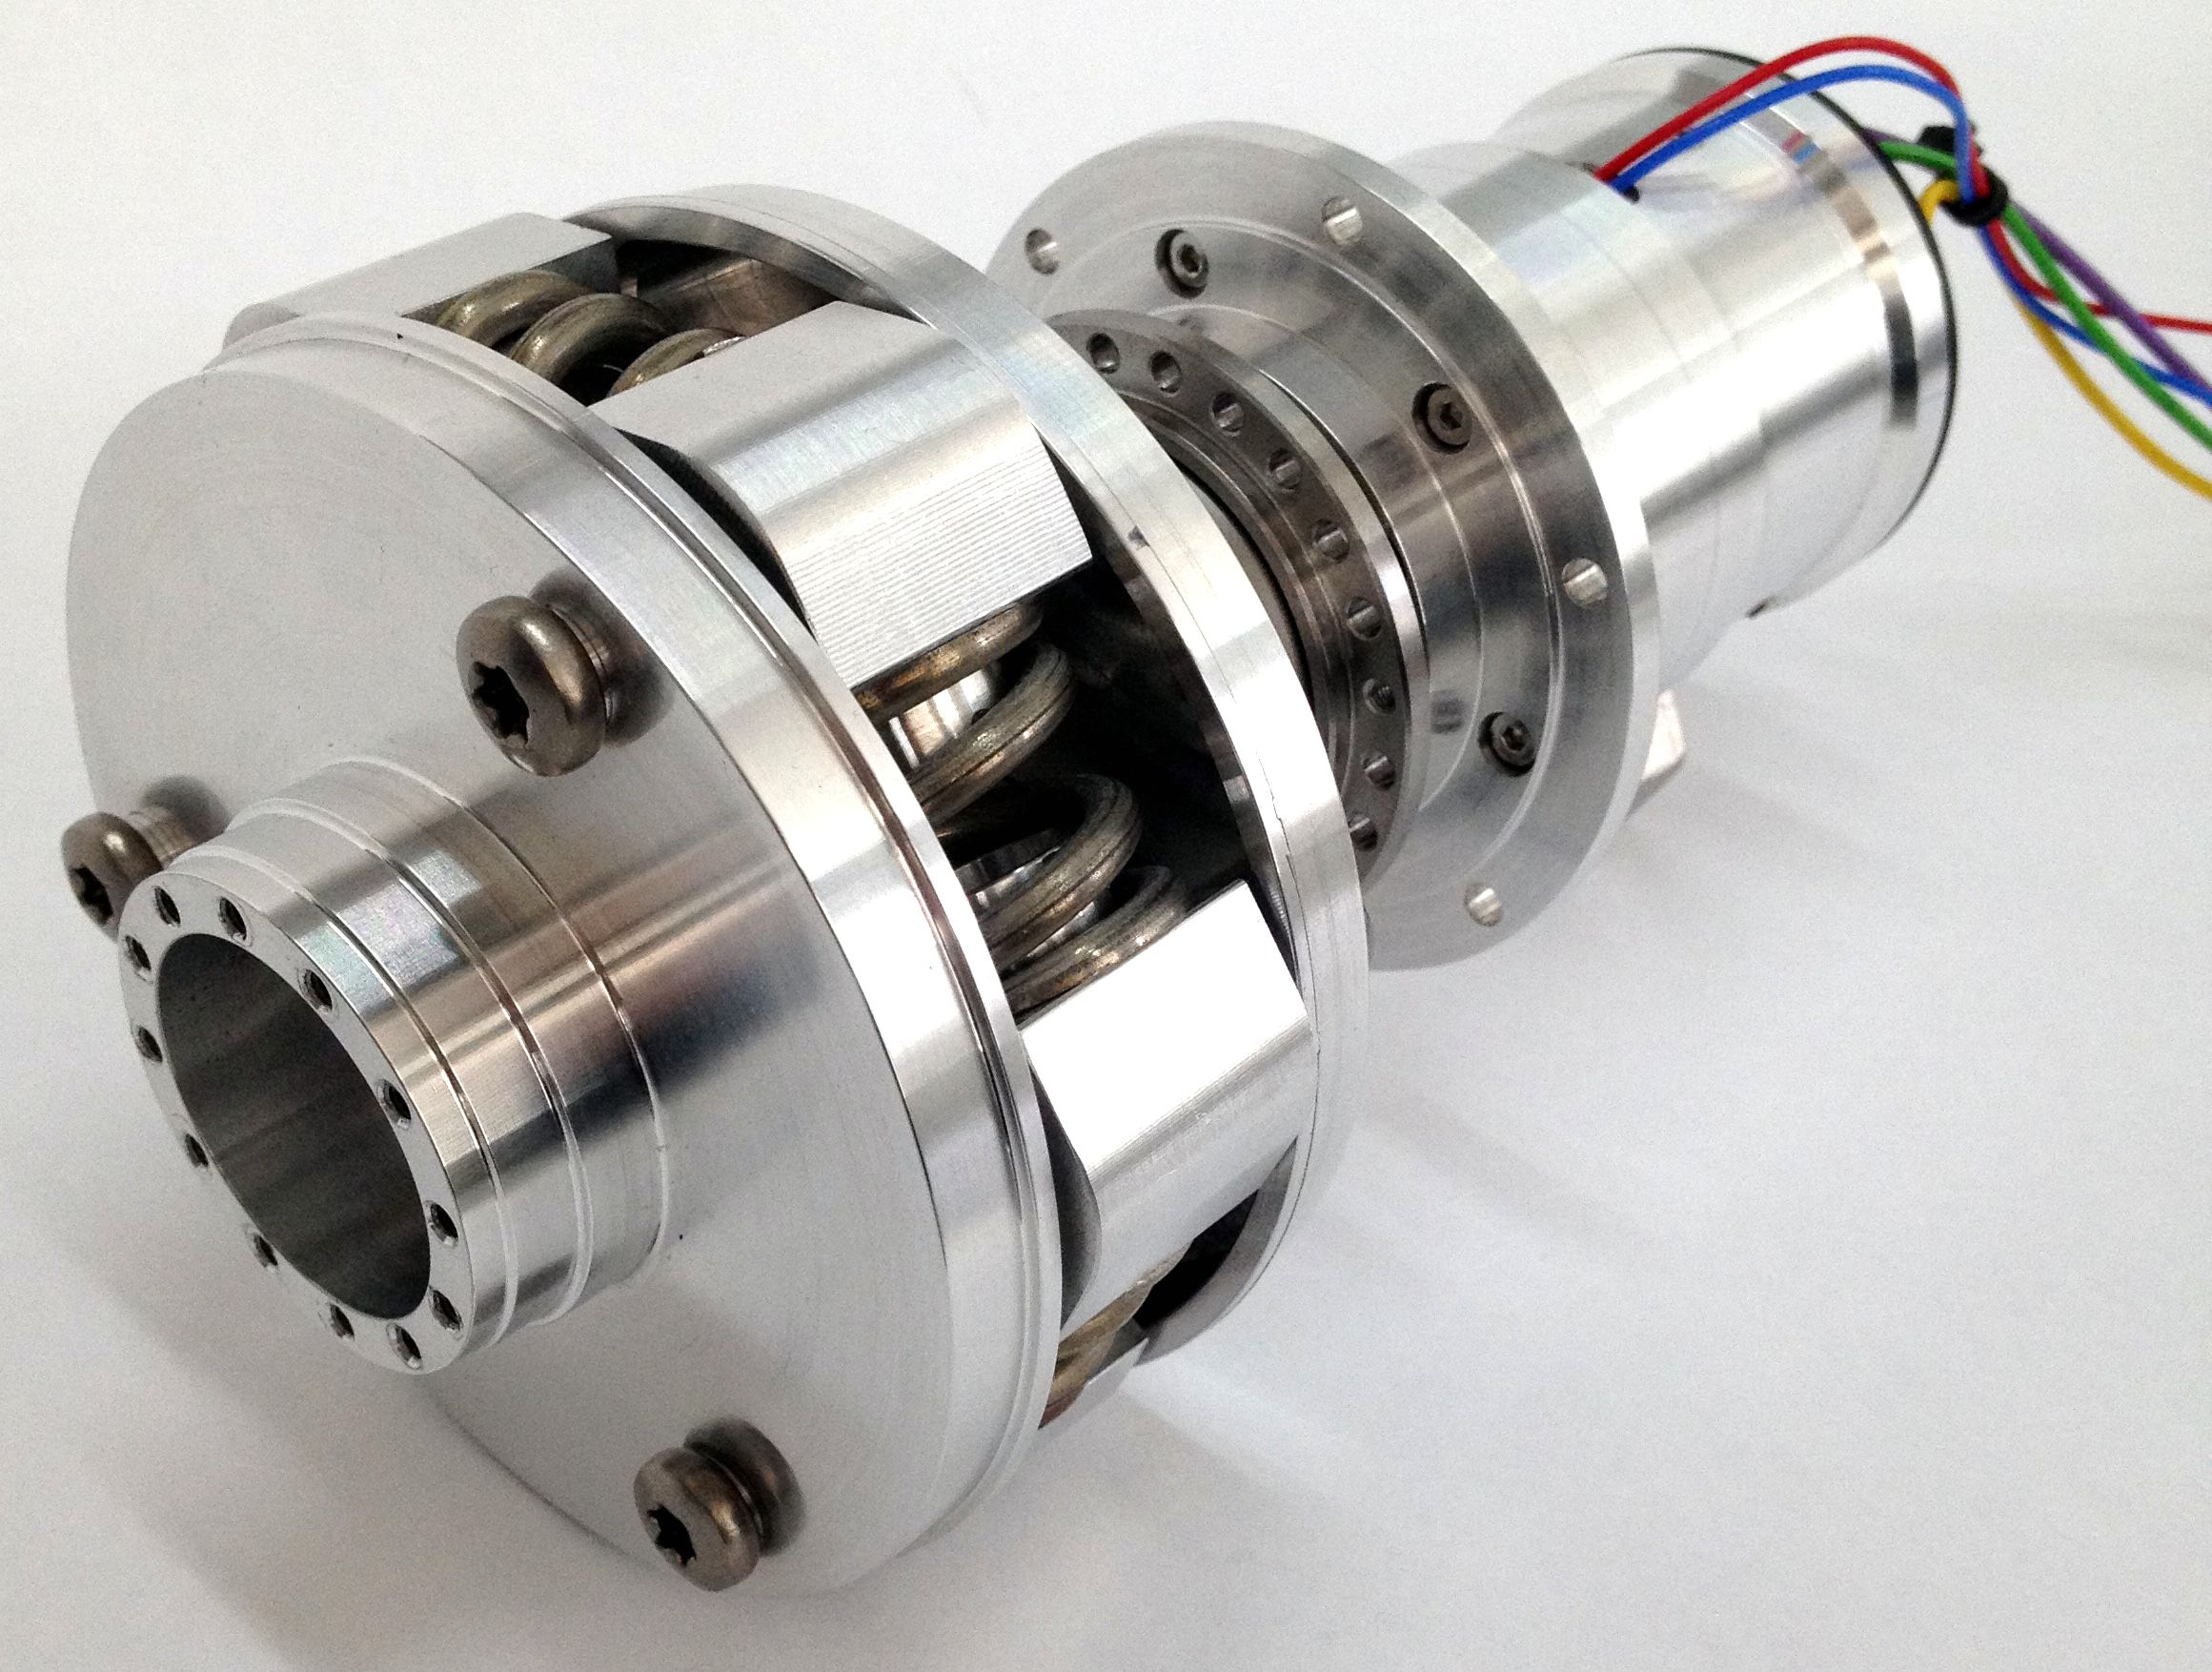
\includegraphics[width=0.4\columnwidth]{./images/50NmJoint_WithoutHousing_07.jpg}
%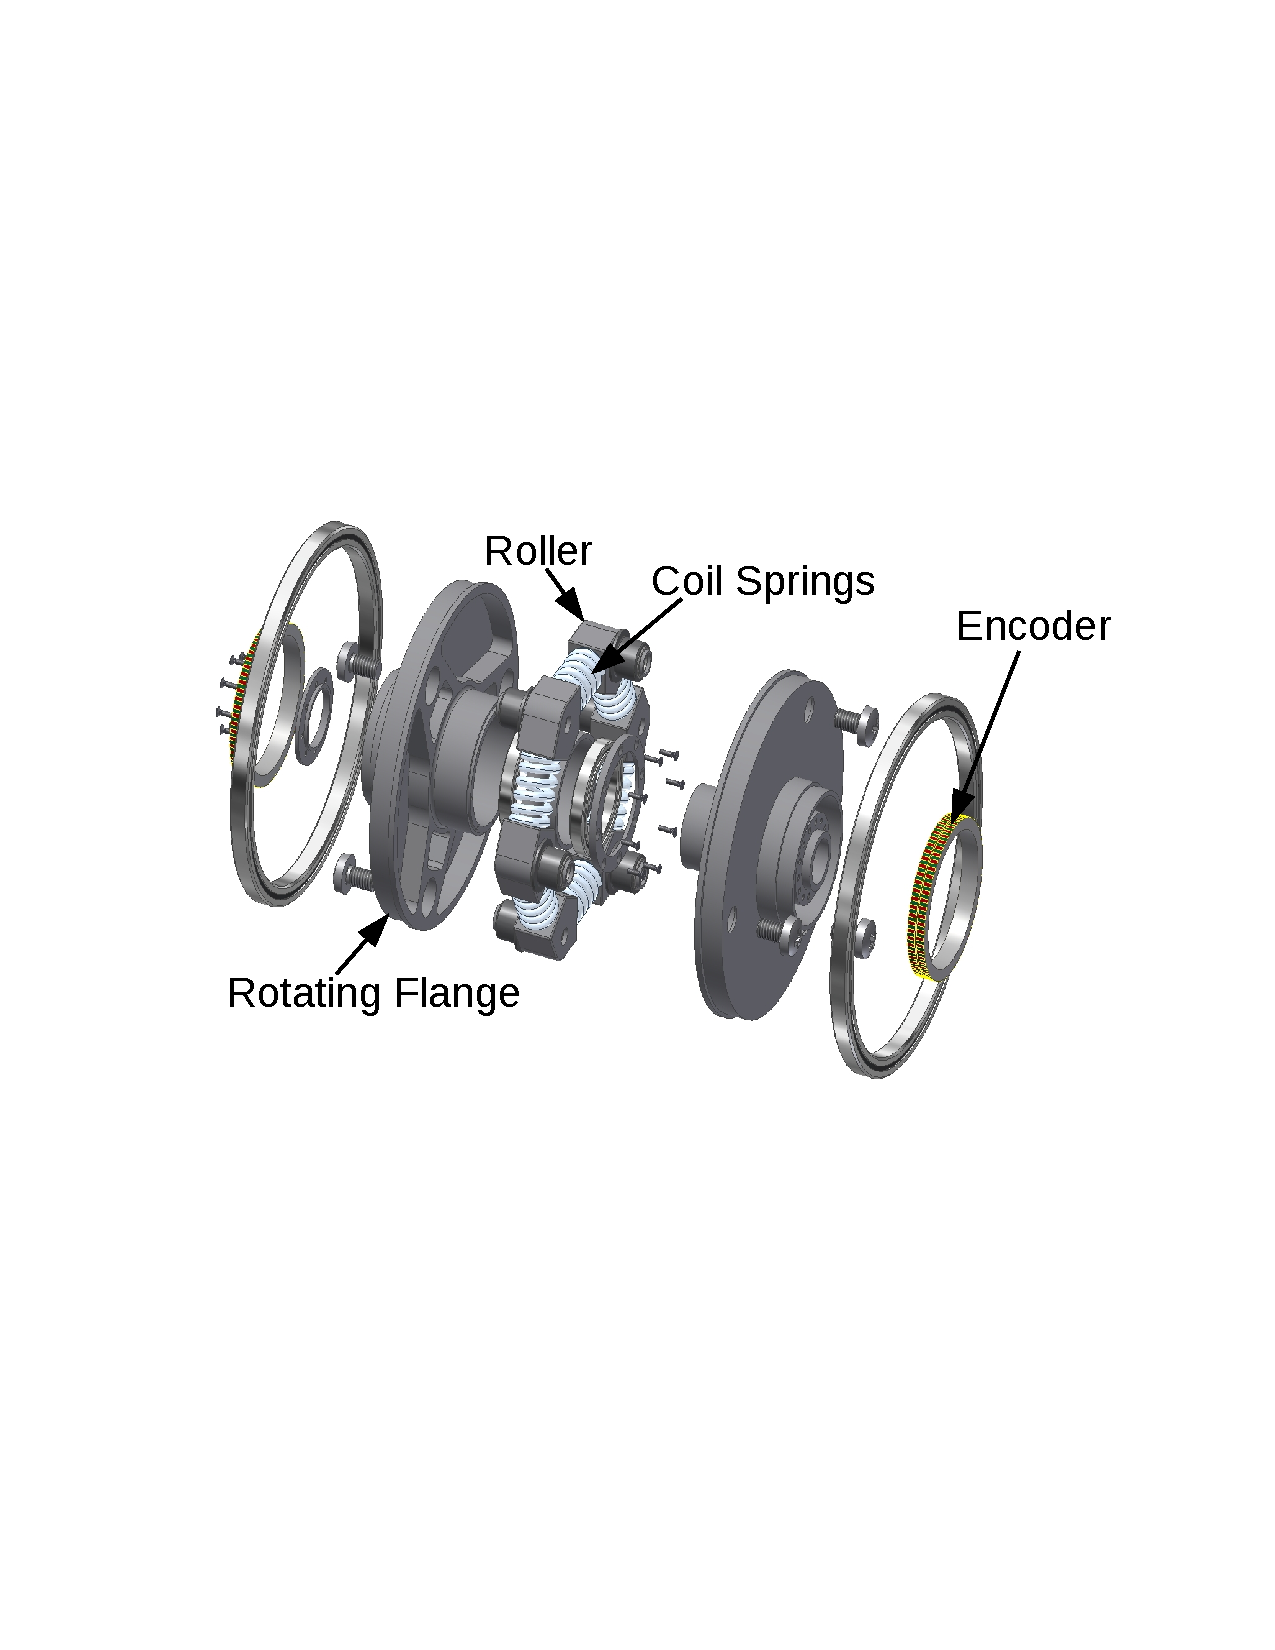
\includegraphics[clip, trim=2.5cm 9.5cm 2.5cm 8.5cm,width=0.5\columnwidth]{./images/Spring_coupling_structure.pdf}
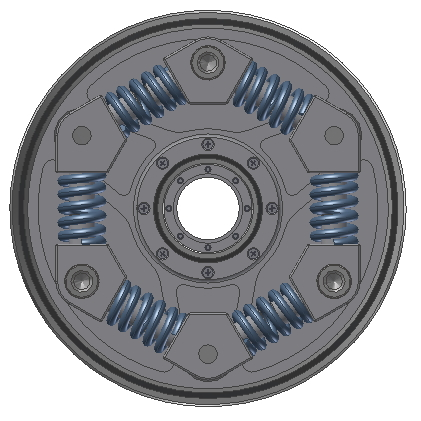
\includegraphics[width=0.3\columnwidth]{./images/Spring_Coupling_03.jpg}
 \caption{\textit{left:} FourByThree 50Nm-Actuator. \textit{right:} Elastic element based on coil springs.}
 \label{fig:4by3_50Nm_actuator}
\end{figure}
%%%%%%%%%%%%%%%%%%%%%%%%%%%%%%%%%%%%%%%%%%%%%%%%%%%%%%%%%%%%%%%%%%%%%%%%%%%%%%%

As shown in Figure \ref{fig:4by3_50Nm_actuator},  coil springs are used and each single spring is a linear element. However due to the internal friction and different pre-compression during assembly, the torque-deflection curve of the overall spring module is nonlinear. Figure~\ref{fig:Spring_torque_curve_2D} shows the result of an experiment used to demonstrate the nonlinearity of the spring coupling. In this experiment, the elastic actuator is controlled to a fixed rotation angle in position control. An external force/torque sensor (Lorenz-DF30) is employed to provide a torque ground truth in a range of -50Nm to +50Nm with an accuracy class of 0.05\%.  The motor is fixed on a test bed, the external torque is externally applied to the spring through the link lever in both directions. As the plot shows, the torque-deflection model of the spring presents a hysteresis characteristic, where a simple linear regression line is a poor choice of representation.

%%%%%%%%%%%%%%  Figure: static analysis of the spring coupling  %%%%%%%%%%%%%%%%%%%%%%%%% 
\begin{figure}[htb]
\centering
\advance\leftskip 0.3cm
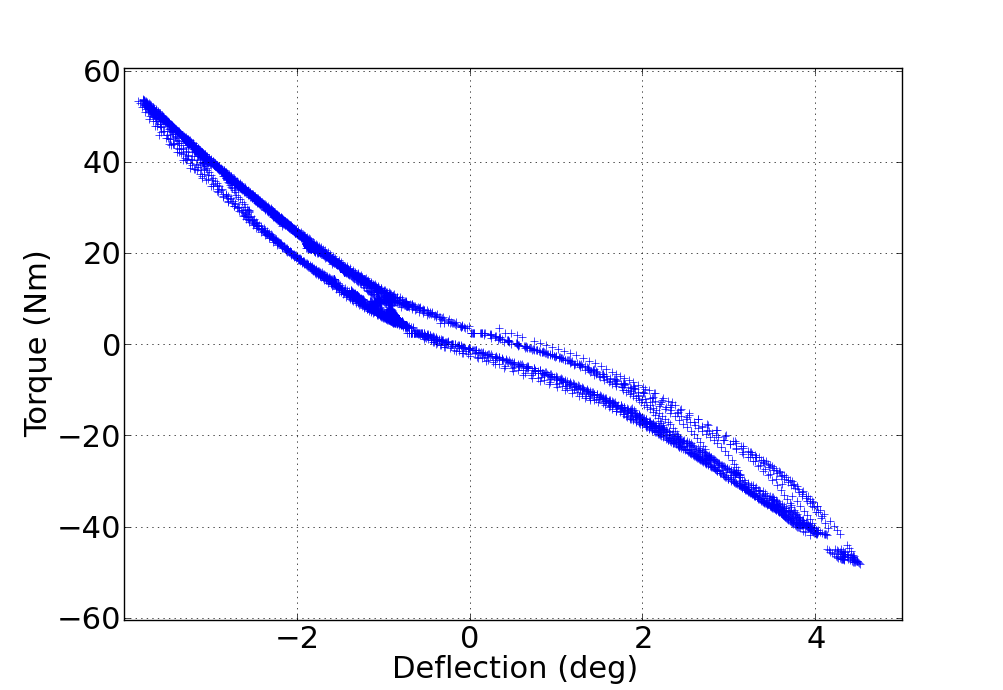
\includegraphics[width=0.9\columnwidth]{./images/spring_static_analysis.png}
 \caption{Torque to deflection curve of the spring coupling. The output torque is measured with an external force/torque sensor and the deflection is measured by computing the difference of two absolute encoders at both sides of the spring.}
 \label{fig:Spring_torque_curve_2D}
\end{figure}
%%%%%%%%%%%%%%%%%%%%%%%%%%%%%%%%%%%%%%%%%%%%%%%%%%%%%%%%%%%%%%%%%%%%%%%%%%%%%%%
